% Source: graduate-coursework/Research/Intro_to_Agents/handouts/Part4_Planning_Workflow.tex

\documentclass[border=4pt]{standalone}
\usepackage{graphicx}
\usepackage{tikz}
\usepackage{xcolor}
\usetikzlibrary{shapes.geometric, arrows.meta, positioning, calc, fit, backgrounds}

\definecolor{UofSCGarnet}{HTML}{73000A}
\definecolor{UofSCBlack}{HTML}{000000}
\definecolor{UofSCWhite}{HTML}{FFFFFF}
\definecolor{UofSCAtlantic}{HTML}{466A9F}
\definecolor{UofSCCongaree}{HTML}{1F414D}
\definecolor{UofSCHorseshoe}{HTML}{65780B}
\definecolor{UofSCRose}{HTML}{CC2E40}
\definecolor{UofSCDarkGarnet}{HTML}{570008}
\definecolor{UofSC90Black}{HTML}{363636}
\definecolor{UofSC70Black}{HTML}{5C5C5C}
\definecolor{UofSC50Black}{HTML}{A2A2A2}

\tikzset{
    box/.style={
        draw=UofSCBlack,
        fill=#1,
        minimum width=2.5cm,
        minimum height=0.8cm,
        text=UofSCWhite,
        font=\small\bfseries,
        align=center,
        inner sep=4pt
    },
    box/.default=UofSCGarnet,
    lightbox/.style={
        draw=UofSCBlack,
        fill=UofSCWhite,
        minimum width=2.5cm,
        minimum height=0.8cm,
        text=UofSCBlack,
        font=\small,
        align=center,
        inner sep=4pt
    },
    arrow/.style={
        ->,
        >=Stealth,
        thick,
        UofSCBlack
    },
    bigarrow/.style={
        ->,
        >=Stealth,
        line width=1.5pt,
        UofSCGarnet
    },
    phase/.style={
        draw=UofSCBlack,
        fill=#1,
        minimum width=3cm,
        minimum height=1cm,
        text=UofSCWhite,
        font=\bfseries,
        align=center
    },
    phase/.default=UofSCGarnet,
    subphase/.style={
        draw=UofSC70Black,
        fill=UofSCWhite,
        minimum width=2.8cm,
        minimum height=0.6cm,
        text=UofSCBlack,
        font=\scriptsize,
        align=center
    },
    cyclebox/.style={
        draw=UofSCBlack,
        line width=1.5pt,
        fill=#1,
        minimum width=2cm,
        minimum height=1.2cm,
        text=UofSCWhite,
        font=\bfseries,
        align=center
    },
    cyclebox/.default=UofSCGarnet
}

\begin{document}
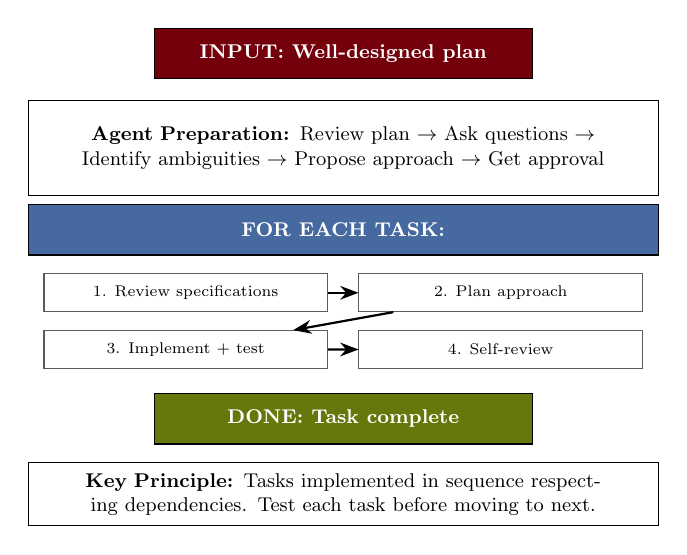
\begin{tikzpicture}[scale=0.8, transform shape]
        % Input
        \node[box=UofSCGarnet, minimum width=6cm] (input) at (0,3.5) {INPUT: Well-designed plan};

        % Preparation box
        \node[lightbox, minimum width=10cm, minimum height=1.5cm, text width=9.5cm] at (0,2) {
            \textbf{Agent Preparation:} Review plan $\rightarrow$ Ask questions $\rightarrow$ Identify ambiguities $\rightarrow$ Propose approach $\rightarrow$ Get approval
        };

        % For each task
        \node[box=UofSCAtlantic, minimum width=10cm] at (0,0.7) {FOR EACH TASK:};

        % Task steps
        \node[subphase, minimum width=4.5cm] (t1) at (-2.5,-0.3) {1. Review specifications};
        \node[subphase, minimum width=4.5cm] (t2) at (2.5,-0.3) {2. Plan approach};
        \node[subphase, minimum width=4.5cm] (t3) at (-2.5,-1.2) {3. Implement + test};
        \node[subphase, minimum width=4.5cm] (t4) at (2.5,-1.2) {4. Self-review};

        \draw[arrow] (t1) -- (t2);
        \draw[arrow] (t2) -- (t3);
        \draw[arrow] (t3) -- (t4);

        % Output
        \node[box=UofSCHorseshoe, minimum width=6cm] at (0,-2.3) {DONE: Task complete};

        % Key principle
        \node[lightbox, minimum width=10cm, minimum height=1cm, text width=9.5cm] at (0,-3.5) {
            \textbf{Key Principle:} Tasks implemented in sequence respecting dependencies. Test each task before moving to next.
        };
    \end{tikzpicture}
\end{document}
